\section{Statistical Analysis}

% The filename of each non-segmented brain MRI contains the age of the subject. Compute the correlation between brain volume and age as well as between white matter, grey matter ratio and age, and state the model assumptions [5]. For each correlation, compute its statistical significance [5].

% Repeat the same experiments by normalising the brain volume by the total intracranial volume (white matter, grey matter and cerebrospinal fluid) [5]. What conclusions can you drawn from these analyses [10]?

The volume of each segmented tissue for the unsegmented subjects can be calculated using the corresponding NIfTI headers, which contains information about voxel dimensions. The Pearson correlation coefficient has been used to compute the correlations between age and tissue volumes. This model assumes that the variables are normally distributed and that relations between them are linear. Also, perfect segmentations are assumed for the statistical analysis.

Once the volumes have been calculated, they can be compared to the subjects ages, as shown in Figure \ref{fig:volumes-correlations}, where normalised volumes mean tissue volume divided by intracranial volume (ICV), which is the addition of CSF, GM and WM volumes. No correlation has been found between the ages and WM/GM ratio ($\rho = 0.09$, $p = 0.706$).

The most significant correlation ($\rho = -0.52$, $p = 0.018$) is the one for age vs. normalised brain volume (i.e. (GM + WM) / ICV). A negative Pearson correlation ratio indicates that the volume of the brain compared to the ICV decreases with age. This seems to be due to the fact that WM is also reduced with age ($\rho = -0.44$, $p = 0.055$), although this relation is less significant. Results in first row of Figure \ref{fig:volumes-correlations} indicate that absolute brain volume is independent of age. For example, the brain of a small young person might be smaller than the brain of an big old person. However, the older brain is likely to be smaller with respect to the ICV, i.e. it has shrinked over time.

\begin{figure}
  \centering
  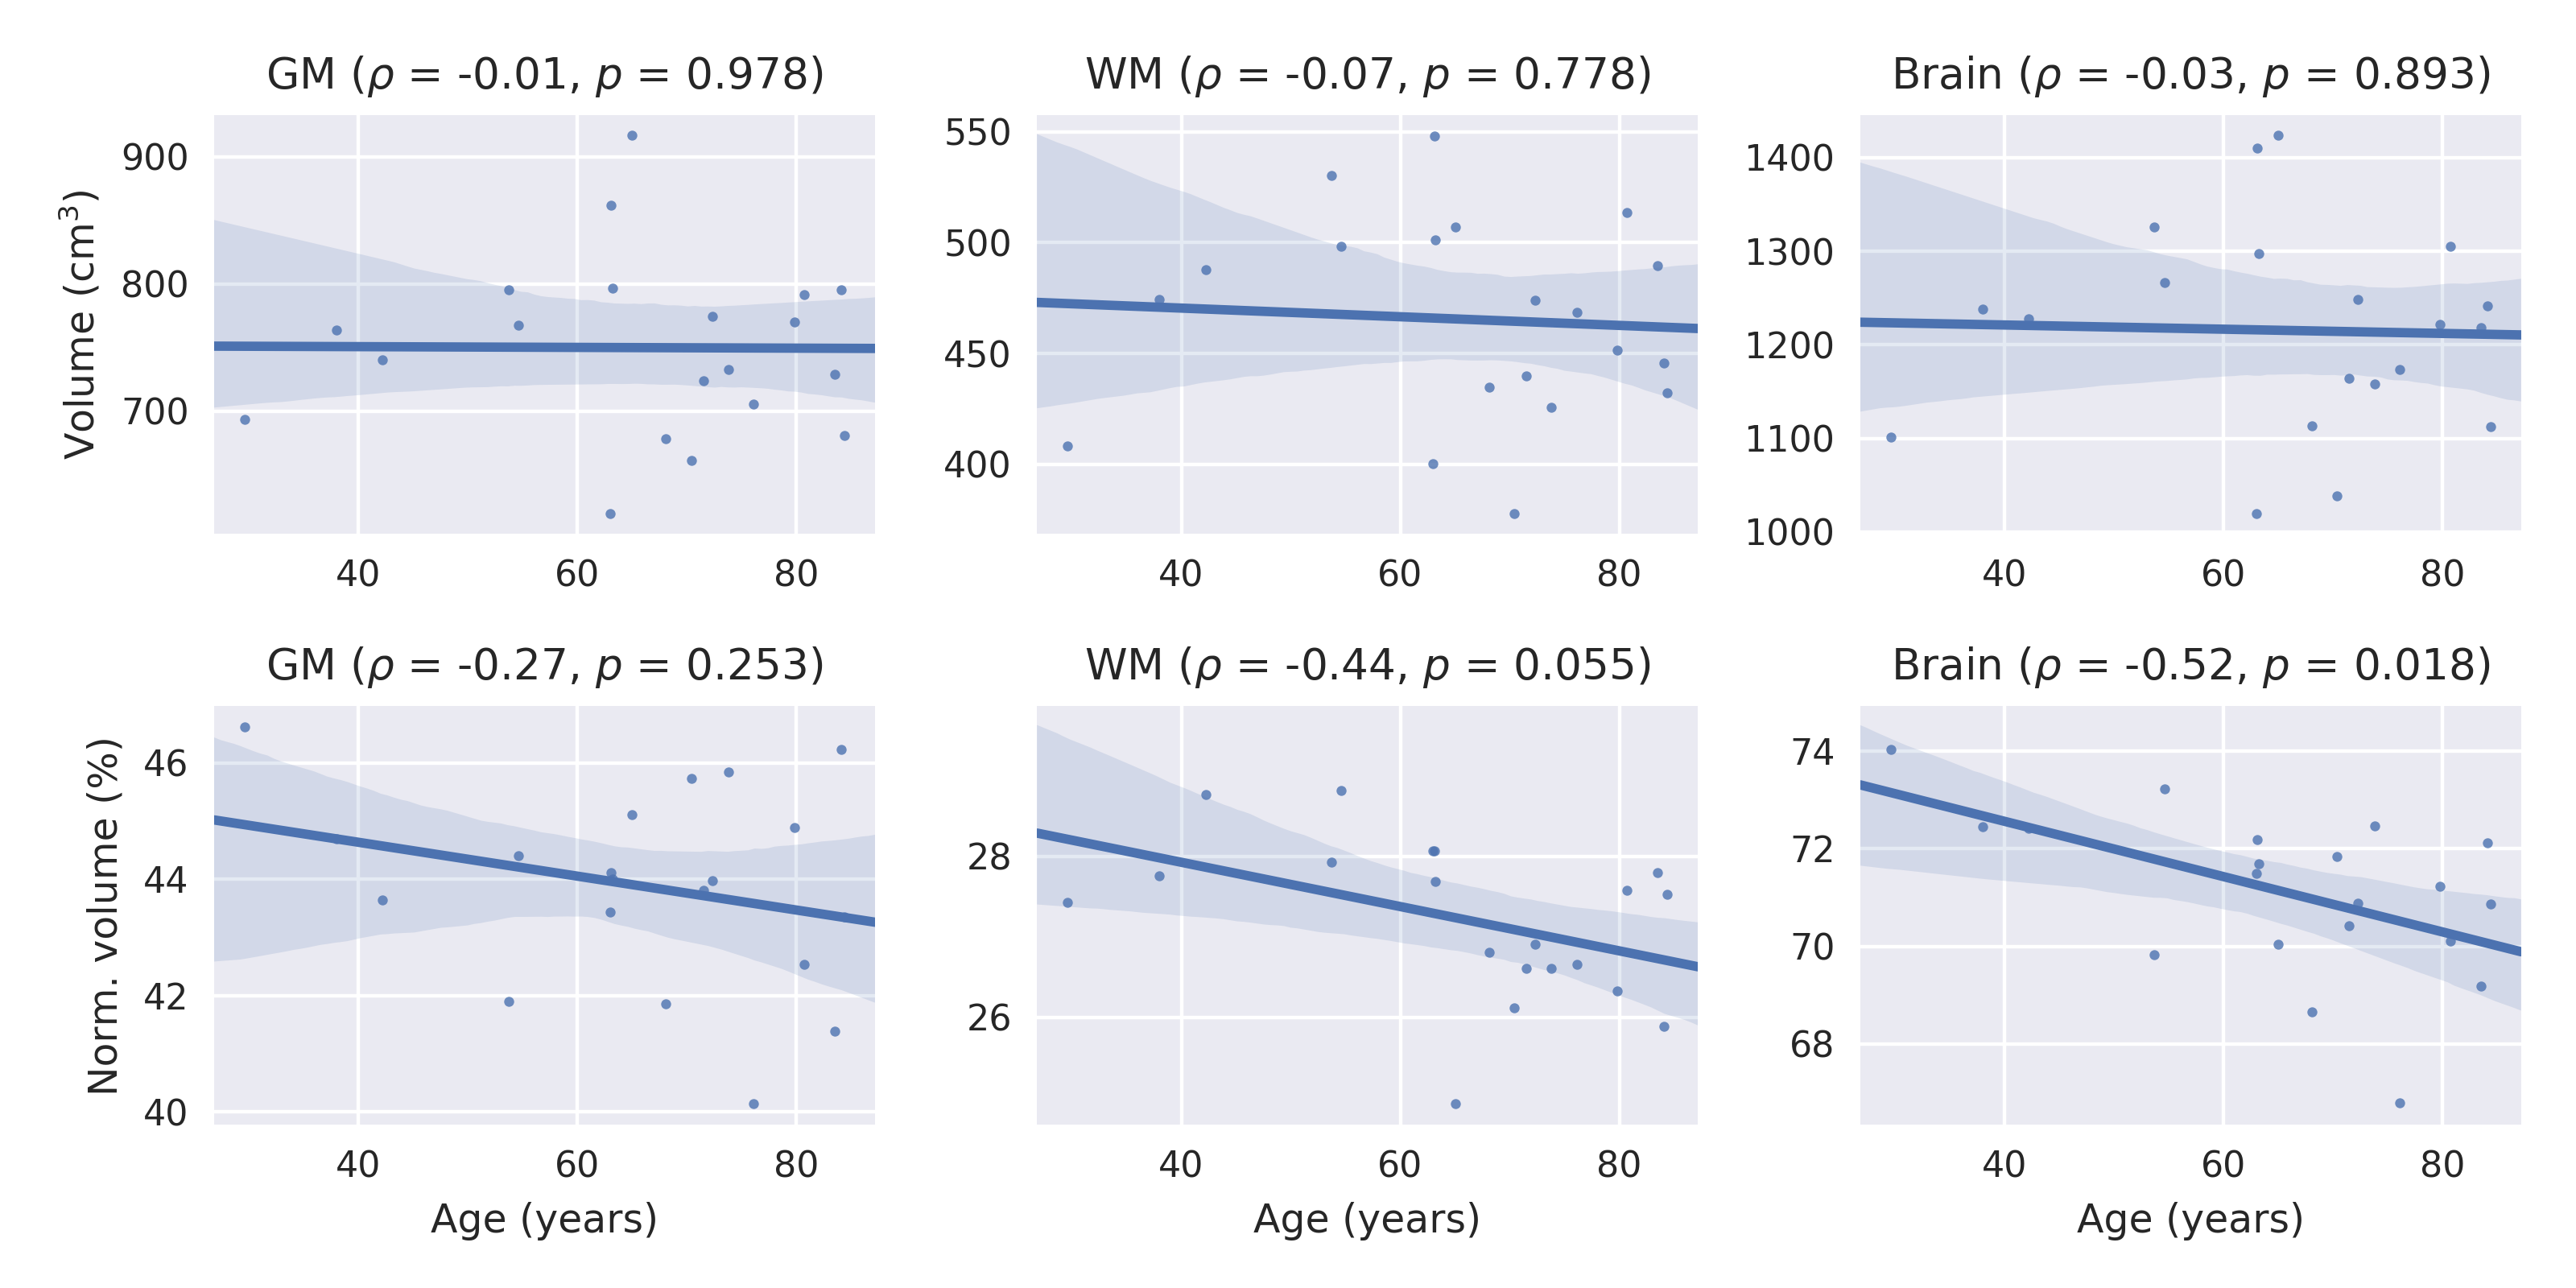
\includegraphics[width=\textwidth]{figures/volumes_stats_pearson}
  \caption{Correlations between age and segmented tissue volumes. Top row: volumes in cm$^3$; bottom row: normalised volumes (i.e. divided by ICV). Brain volume is calculated as GM volume + WM volume. $\rho$ represents the Pearson correlation coefficient and $p$ is the two-tail p-value for testing non-correlation. Dots represent individual subjects; lines represent regression models; shaded areas represent 95 \% confidence intervals.}
  \label{fig:volumes-correlations}
\end{figure}

The confidence in a statistical analysis with only 20 subjects is small. To increase the statistical power of the study, the same measurements have been performed on the IXI dataset \cite{noauthor_ixi_nodate}, composed on almost 600 MR images from normal, healthy subjects. Figures~\ref{fig:ixi-all} and~\ref{fig:ixi-ratio} show the results. For this data, there is a strong correlation between age and reduced normalised GM volume, while there are no significant changes in normalised WM volume. These two findings are coherent with the negative correlation between age and normalised brain volume (if WM stays the same and GM is reduced, brain is reduced) and positive in the case of age vs. WM/GM ratio. The absolute GM and brain volumes also seem to be smaller with age, but the correlation is weaker.


\begin{figure}
  \centering
  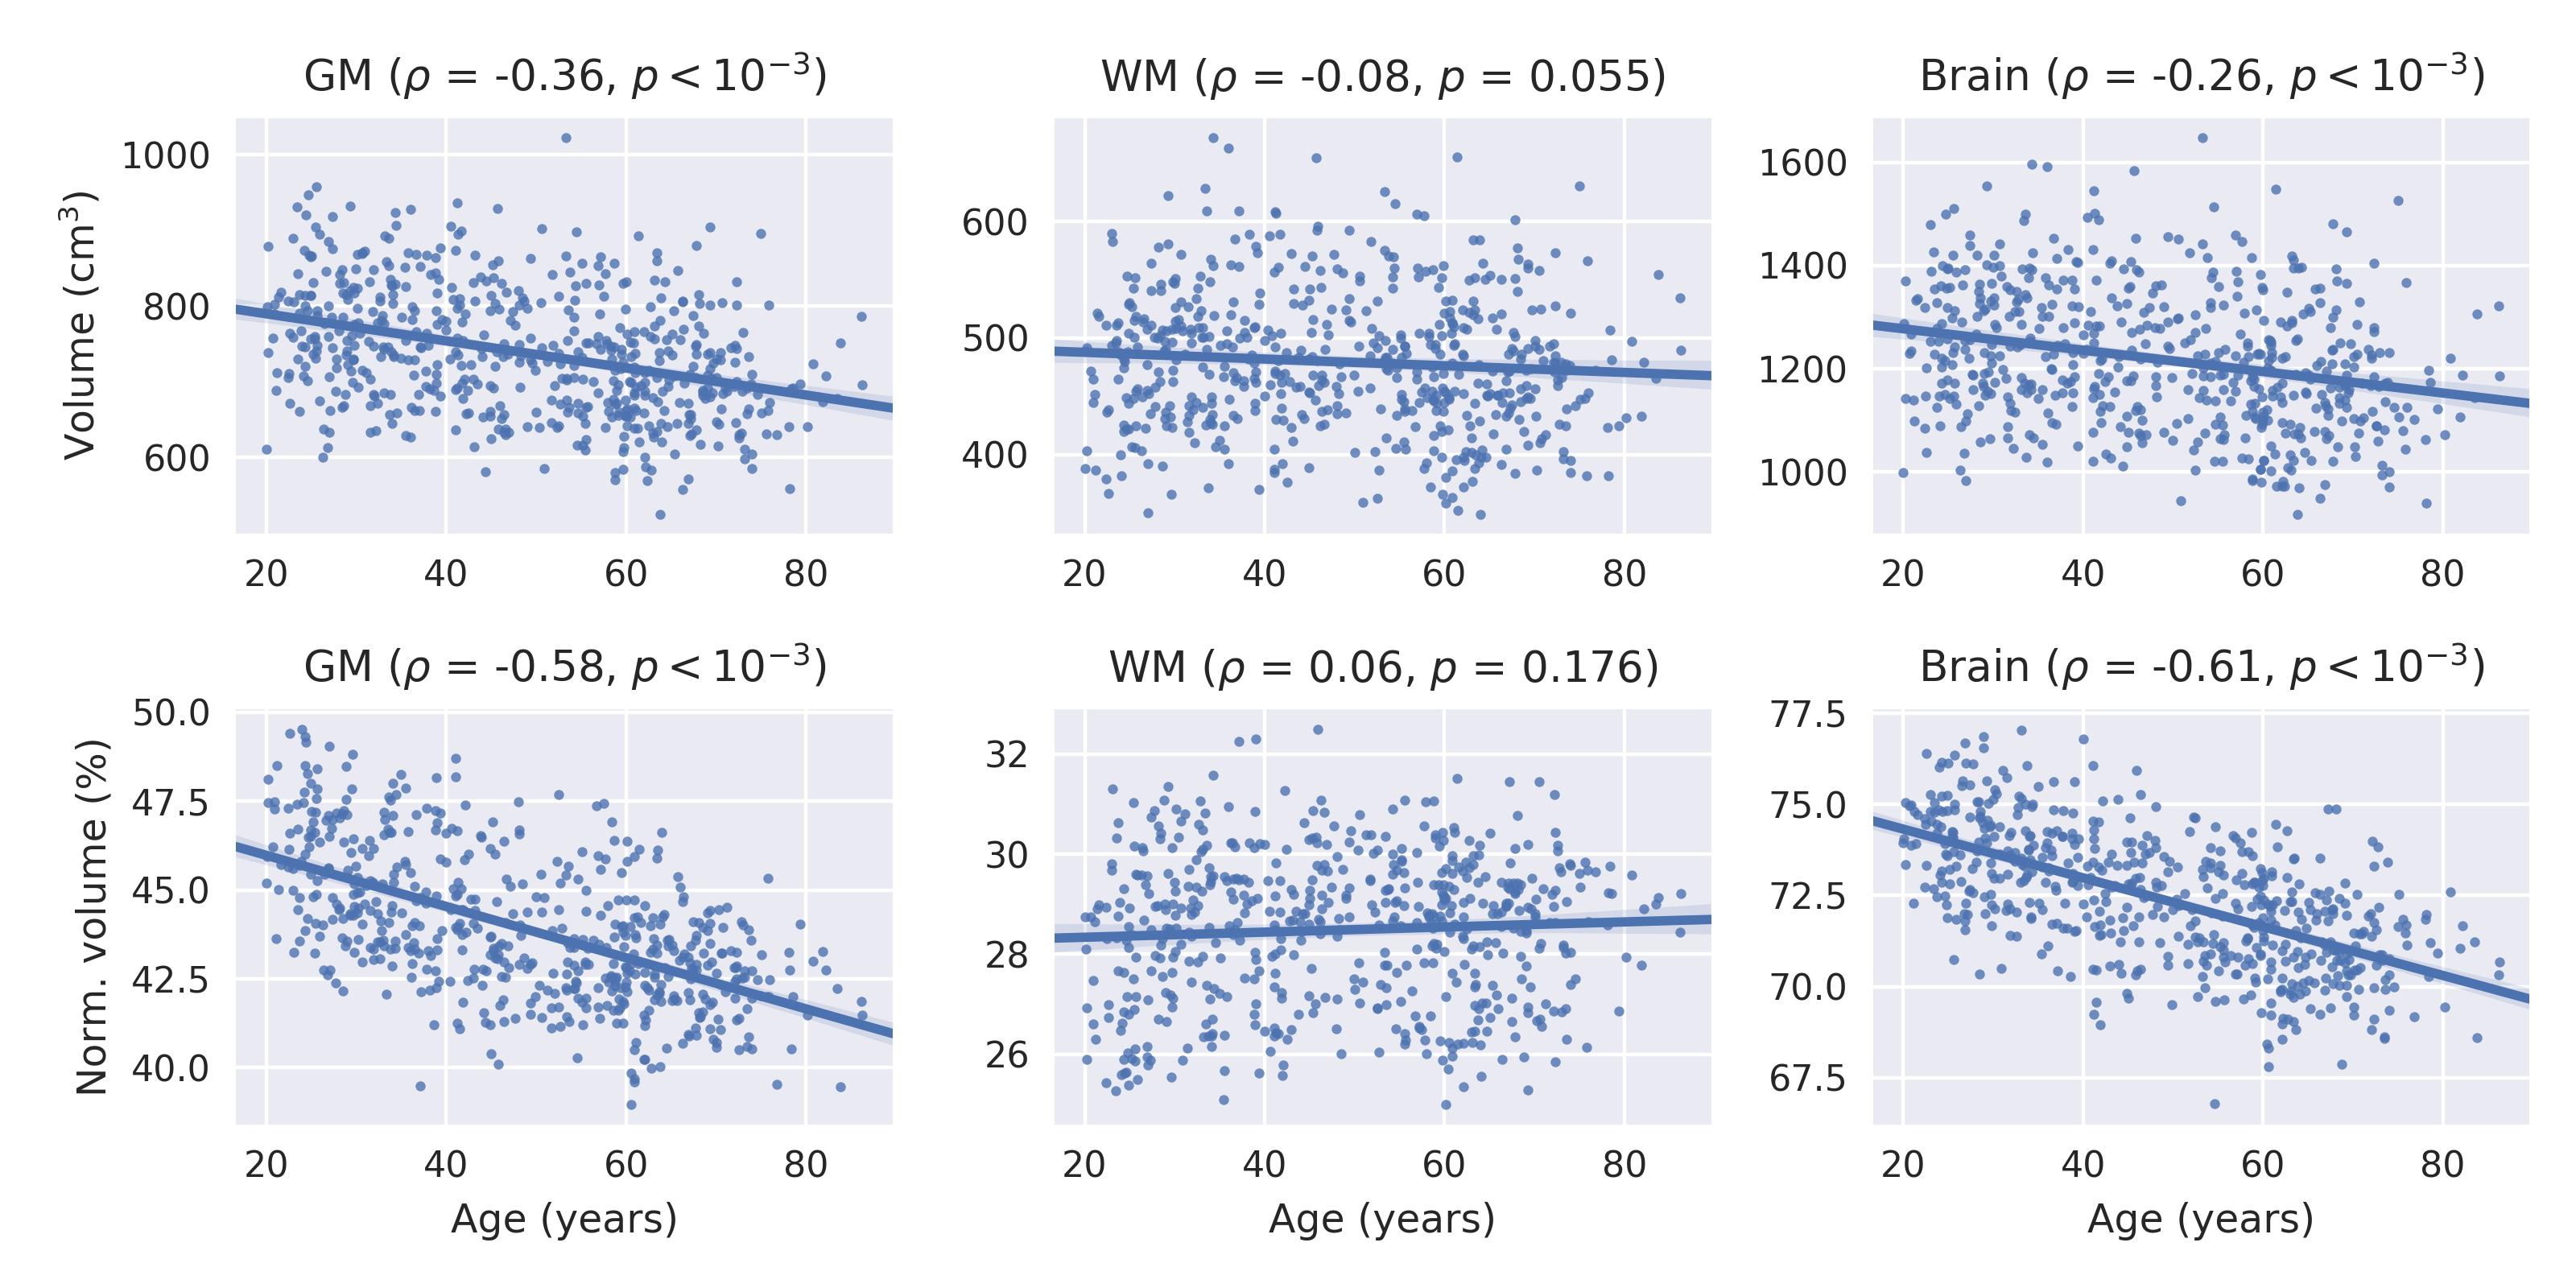
\includegraphics[width=\textwidth]{figures/volumes_stats_pearson_ixi}
  \caption{Correlations between age and segmented tissue volumes from the IXI dataset. Top row: volumes in cm$^3$; bottom row: normalised volumes (i.e. divided by ICV). Brain volume is calculated as GM volume + WM volume. $\rho$ represents the Pearson correlation coefficient and $p$ is the two-tail p-value for testing non-correlation. Dots represent individual subjects; lines represent regression models; shaded areas represent 95 \% confidence intervals.}
  \label{fig:ixi-all}
\end{figure}

\begin{figure}
  \centering
  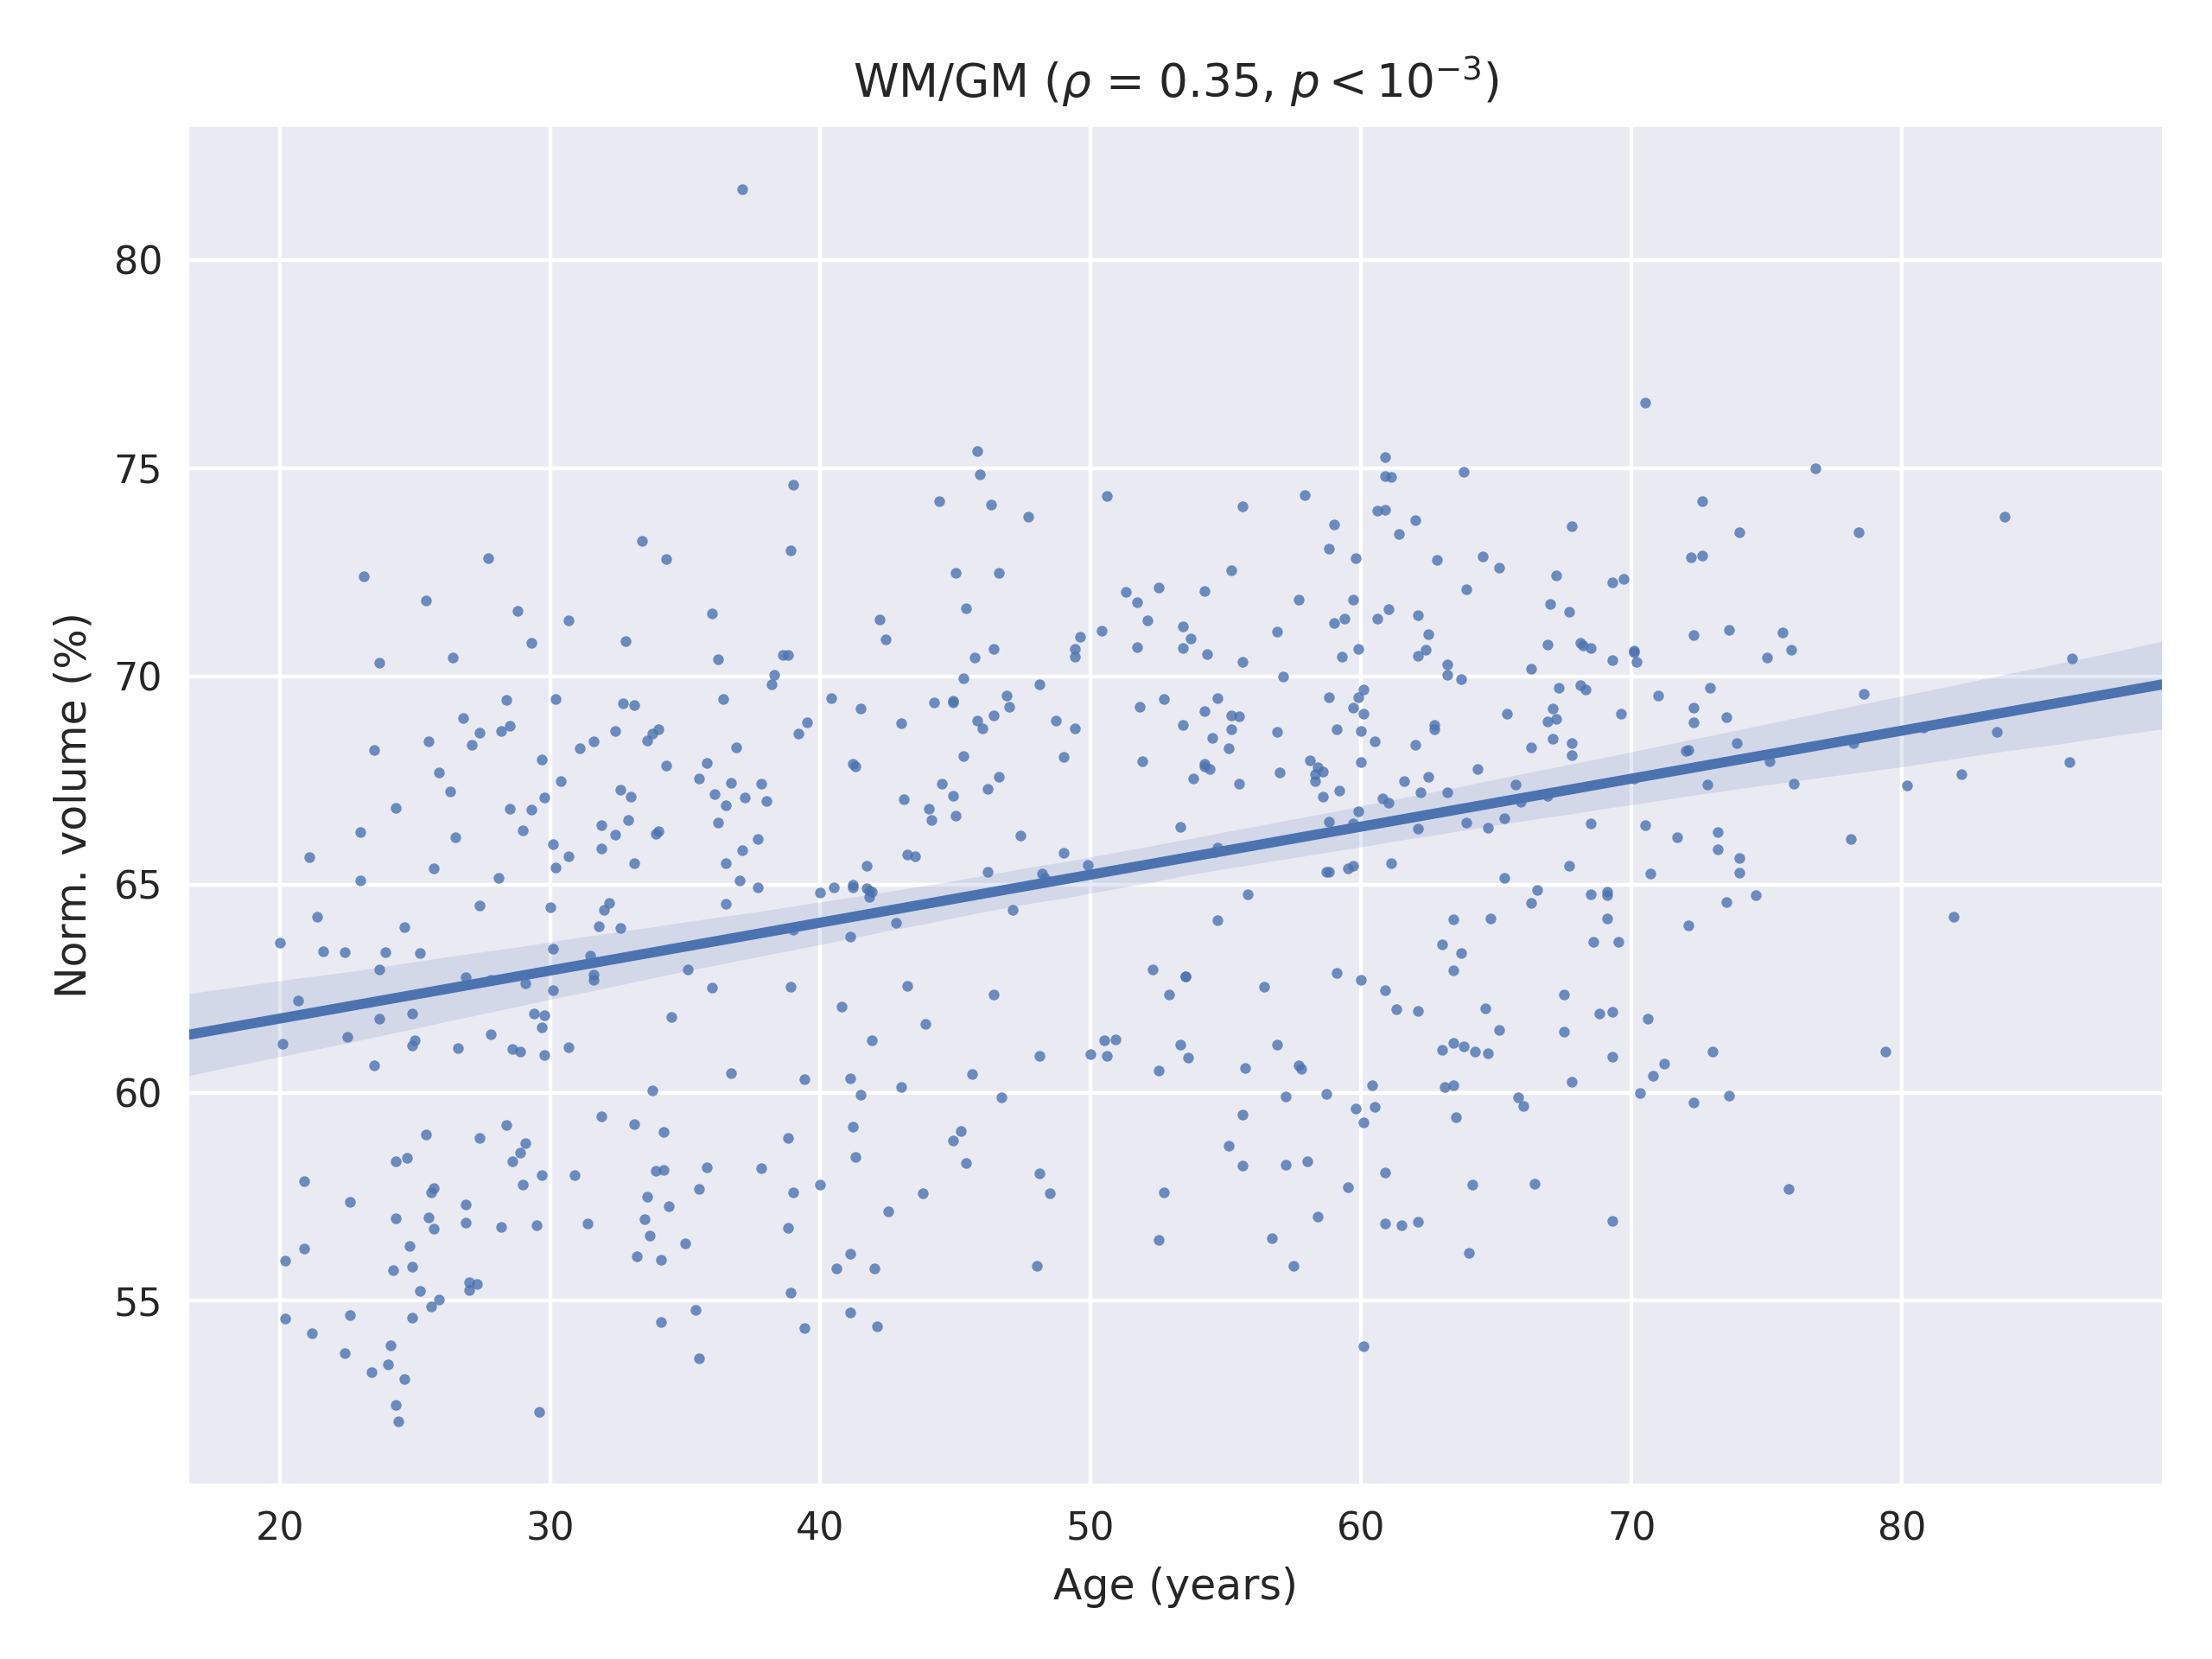
\includegraphics[width=0.7\textwidth]{figures/volumes_stats_pearson_wm_gm_ixi}
  \caption{Correlation between age and WM/GM ratio from the IXI dataset. $\rho$ represents the Pearson correlation coefficient and $p$ is the two-tail p-value for testing non-correlation. Dots represent individual subjects; the line represents the regression model; the shaded area represents the 95 \% confidence interval.}
  \label{fig:ixi-ratio}
\end{figure}
